\documentclass[11pt, oneside]{article}   	% use "amsart" instead of "article" for AMSLaTeX format
\usepackage{geometry}                		% See geometry.pdf to learn the layout options. There are lots.
\geometry{a4paper}                   		% ... or a4paper or a5paper or ... 
%\geometry{landscape}                		% Activate for rotated page geometry
%\usepackage[parfill]{parskip}    		% Activate to begin paragraphs with an empty line rather than an indent
\usepackage{graphicx}				% Use pdf, png, jpg, or eps§ with pdflatex; use eps in DVI mode
								% TeX will automatically convert eps --> pdf in pdflatex		
\usepackage{amssymb}

\graphicspath{ {./images/} } 				

%SetFonts

%SetFonts


\title{Ricerca operativa}
\author{941519}
%\date{}							% Activate to display a given date or no date

\begin{document}
\maketitle
\section{Programmazione lineare}
\subsection{Componenti}
\subsection{Dalla forma generale alla forma alle uguaglianze}
\begin{itemize}
\item I termini noti nella funzione maximize/minimize possono essere trascurati per poi essere reintrodotti alla fine dell'esercizio (è solo traslazione)
\item Quando si fa un maximize, si usa $\leq$, quando si fa minimize di fa $\geq$
\end{itemize}
\subsection{Interpretazione geometrica della PL}
\begin{itemize}
\item Ogni vincolo di uguaglianza corrisponde ad un iperpiano
\item Ogni vincolo di disuguaglianza corrisponde ad un semispazio
\item L'intersezione di semispiazi è un poliedro
\item Le soluzioni ammissibili giacciono su un fascio di iperpiani paralleli, caratterizzati dalla loro \emph{direzione di ottimizzazione}
\end{itemize}
\subsubsection{Iperpiano e poliedro}
\subsection{Eliminazione di vincoli di uguaglianza, variabili libere}
\subsection{Forma standard}
\begin{itemize}
\item La funzione obbiettivo è posta in forma di minimizzazione
\item Tutti i vincoli di disuguaglianza vengono posti in forma di uguaglianze, introducendo opportune variabili non-negative di scarto/slack (minore uguale) o di surplus (maggiore uguale)
\end{itemize}
\subsubsection{Minimizzazione della forma standard}
\subsubsection{Variabili di scarto e di surplus}
\subsection{Teorema fondamentale della PL}
Dato un problema lineare in forma standard:
\begin{itemize}
\item Se esiste una soluzione ammissibile, esiste anche una soluzione ammissibile di base
\item Se esiste una soluzione ottima, esiste anche una soluzione ottima di base.
\end{itemize}

\subsection*{Le forme di un problema di PL}
Le 4 forme di un problema di PL sono:
\begin{itemize}
\item Forma generale
\item Forma alle disuguaglianze
\item Forma alle standard
\item Forma canonica
\end{itemize}

\section{L'algoritmo del Simplesso}
\subsection{Forma canonica}
\begin{itemize}
\item I coefficienti nelle variabili di base formano una matrice identità
\item Le variabili di base non compaiono nella funzione obbiettivo
\item Una forma canonica è forte se tutti i termini noti sono $\geq 0$
\end{itemize}
\subsection{Il tableau}
\subsection{L'algoritmo fondamentale dell'algoritmo del simplesso}
\begin{enumerate}
\item Verifica di inammissibilità
\item Trovare una soluzione ottima, o determinare un problema come illimitato
\end{enumerate}
\subsection{Passo di pivot}
\begin{itemize}
\item Consiste nel cambio di base, una variabile in base esce dalla base, e una variabile fuori base entra in base. Geometricamente consiste nel spostarci lungo uno spigolo
\item Si sceglie un pivot positivo (elemento in riga) su una colonna fuori base
\item Si divide la riga $r$ per il pivot
\item Sottrarre ad ogni riga $i \neq r$ la riga $r$ moltiplicata per $a_{ic}$
\item In questo modo ci troviamo con un tableau nuovo, con una riga nuova in base, e con la colonna che corrispondeva al pivot fuori base.
\end{itemize}


\subsection{Regole di scelta della colonna e della riga}
\subsubsection{Scelta della colonna}
Per scegliere la colonna possono essere utilizzate diverse strategie, a patto che si evitino cicli infiniti nel caso di soluzioni degeneri
\begin{itemize}
\item scegliere la colonna con variabile (numero sopra) con costo ridotto negativo
\item la colonna col minimo coefficiente di costo ridotto
\item la colonna che produce il maggior miglioramento di $z$
\item la prima colonna con costo ridotto negativo, secondo un ordinamento fissato (questo metodo è anche chiamato regola di Bland, si fissa un indice all'inizio dell'algoritmo ad ogni riga/colonna, e si segue l'ordine)
\item una colonna a scelta a caso tra quelle con costo ridotto negativo
\end{itemize}
\subsubsection{Scelta della riga}
Per scegliere la riga bisogna:
\begin{itemize}
\item considerare solo candidati pivot $a_{ij}$ positivi
\item si sceglie quello col minimo rapporto tra il termino noto (a sinistra) $b_i$ ed il candidato pivot (nella matrice) $a_ij$ 
\end{itemize}
Nuovamente applichiamo la regola di Bland per selezionare la riga, quando ci troviamo di fronte ad ambiguità.

\subsection{Test di illimitatezza}
Se non esistono candidati pivot positivi su una colonna con costo ridotto negativo, il problema è detto \emph{illimitato}. In questo caso il problema è probabilmente degenere.

\subsection{Test di inamissibilità}
Se l'inammissibilità rispetto ad un vincolo violato è stata minimizzata, ma il valore della corrispondente rimane negativo, questo dimostra che il problema è inammissibile e l'algoritmo del simplesso termina.

\subsection{Metodo delle variabili artificiali}
%Permette di dimostrare l'inamissibilità di un problema, oppure genera un problema artificiale risolvibile. Il vantaggio è che si può sempre applicare, ma può comportare molti passi di pivot, e genera un tableau più grande dell'originario.

\subsection{Metodo "big M"}
\subsection{Metodo di Balinski-Gomory}

\section{Analisi post-ottimale}
Dopo aver calcolato la soluzione ottima di un problema, è importante valutare la robustezza dei dati (per tenere conto di incertezze, approssimazioni, arrotondamenti)
\subsection{Analisi di sensitività}
Utilizzata per valutare l'intervallo nel quale può variare ogni coefficiente $c_j$ e $b_i$ senza che cambi la base ottima. In particolare vengono considerate le condizioni di ammissibilità (che dipendono solo da $b4) e ottimalità (che dipendono solo da $c$.
\subsubsection{Condizioni di ammissibilità e condizioni di ottimalità}
\subsection{Variazione del coefficiente $b_i$ e del coefficiente $c_i$}
\subsection{Analisi parametrica}
\subsection{Costi ridotti e profitti marginali}


\section{Teoria della dualità}
Si applica su problemi non lineari e problemi nel discreto. Ogni problema di PL, che d'ora in poi chiamiamo problema primale, ammette un problema duale. Le corrispondenze sono definite secondo questo schema:
\subsection{Il problema duale: coppia primale-duale}
\begin{center}
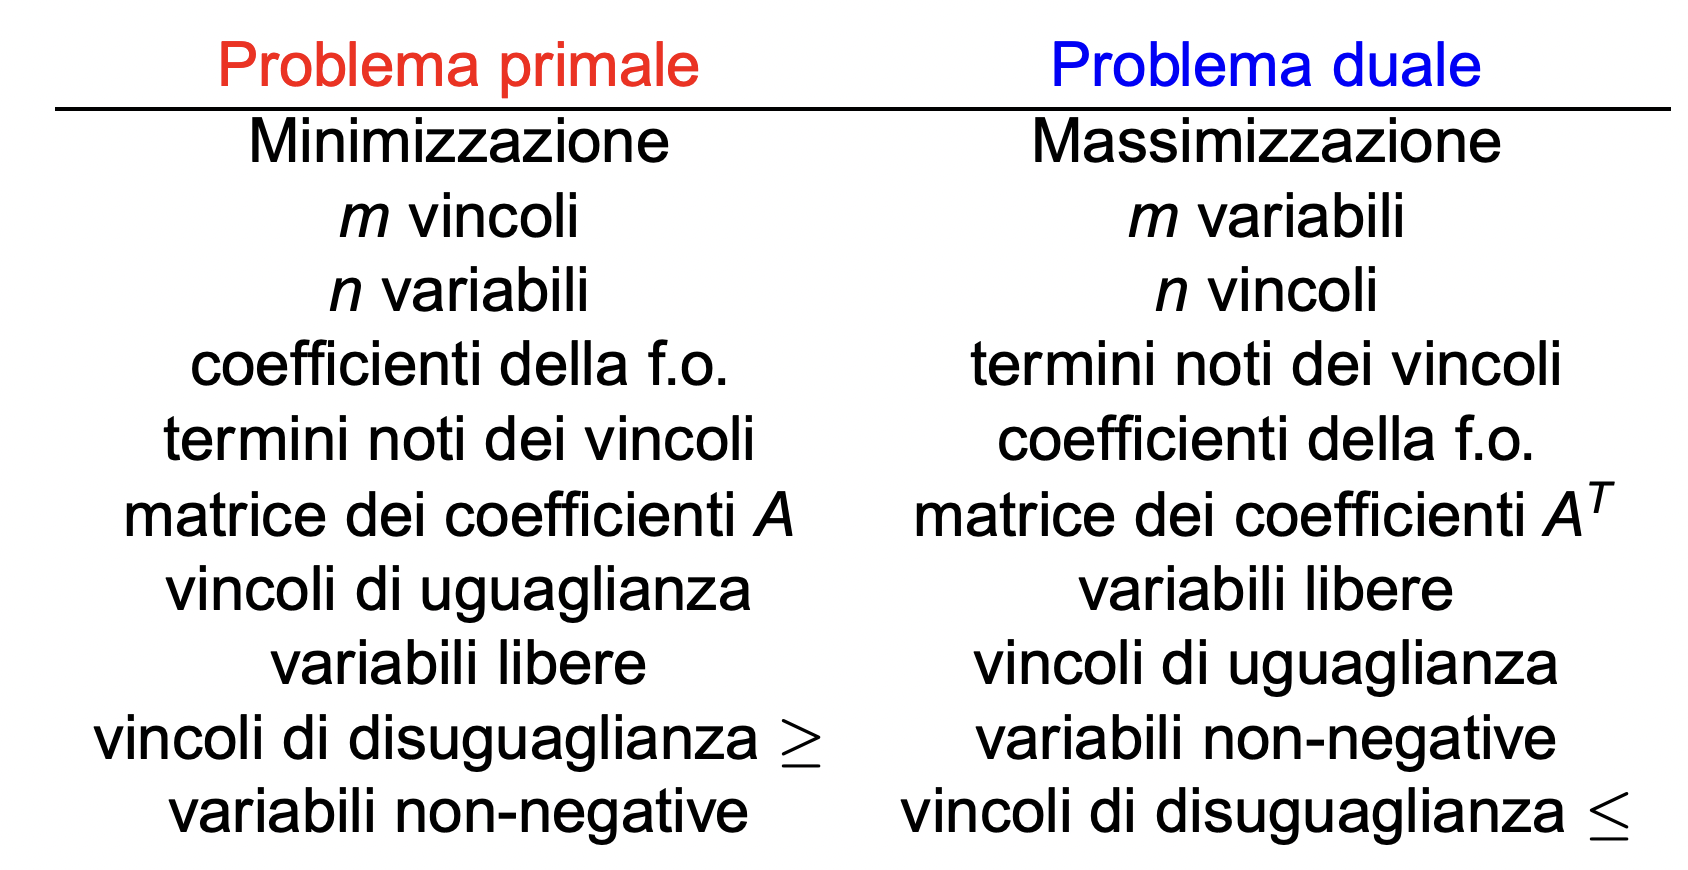
\includegraphics[scale=0.3]{dualita}
\end{center}
\subsection{Teorema della dualità in forma debole}
Data una coppia primale-duale:
\begin{center}
$P:$ maximize $ z(x),$ $s.t. x \in X$ \\
$D:$ minimize $ w(y),$ $s.t. y \in Y$
\end{center}
Per ogni soluzione ammissibile di $x \in X$ di $P$, e per ogni soluzione ammissibile di $y \in Y$ di $D$ si ha
\begin{center}
$z(x) \leq w(y)$
\end{center}
\subsection{Teorema fondamentale dell'algebra}
Dato un sistema di equazioni lineari: \begin{itemize}
\item o esiste un certificato di ammissibilità $x$, la cui esistenza dimostra che il sistema ha una soluzione
\item o esiste un certificato di inammissibilità $y$, la cui esistenza dimostra che il sistema non ha una soluzione
\end{itemize}
\subsubsection{Lemma di Farkas}
Dato un sistema di \emph{equazioni} lineari:
\begin{center}
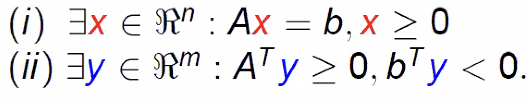
\includegraphics[scale=1]{farkas}
\end{center}
\begin{itemize}
\item i: esiste una soluzione ammissibile del problema
\item ii: non esiste una soluzione ammissibile del problema 
\end{itemize}
\subsubsection{Lemma di Farkas: variante}
Dato un sistema di \emph{disequazioni} lineari:
\begin{center}
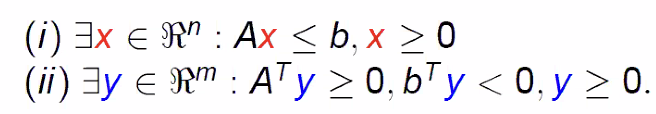
\includegraphics[scale=1]{farkas2}
\end{center}

\subsection{Teorema della dualità in forma forte}
Data una coppia primale-duale, se uno dei due problemi ammette una soluzione ottima finita, allora anche l'altro ammette una soluzione ottima finita, ed i due valori ottimi coincidono.
\begin{center}
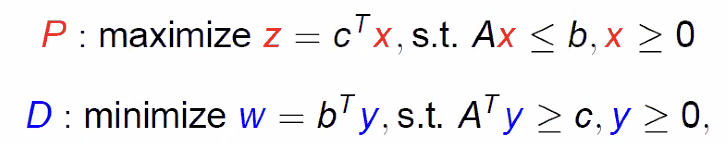
\includegraphics[scale=1]{dualitaf}
\end{center}

\subsection{Teorema fondamentale della dualità lineare}
Data una coppia primale-duale, esiste una sequenza finita di passi di pivot che porta l'algoritmo del simplesos a terminare, portandoci ad uno di quesit 4 casi:
\begin{itemize}
\item soluzione ottima di $P$ e $D$
\item $P$ è illimitato e $D$ è inamissibile
\item $D$ è illimitato e $P$ è inamissibile
\item sia $P$ che $D$ sono inamissibili
\end{itemize}
\subsection{Teorema dello scarto complementare}
Data una coppia primale-duale, la condizione necessaria e sufficiente per l'ottimalità di due soluzioni ammissibili \={x}, \={y}  è che valgono le seguenti equazioni:
\begin{center}
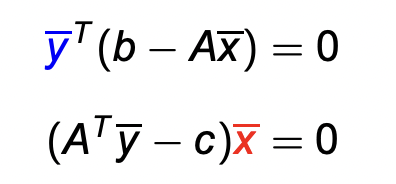
\includegraphics[scale=1]{scarto}
\end{center}
\subsection{L'algoritmo del simplesso duale}
Considerando che i coefficienti di $P$ (primale) e $D$ (duale) sono gli stessi, entrambi i problemi della coppia primale-duale possono essere rappresentati sullo stesso tableau.\\

L'algoritmo del simplesso duale funziona lavorando sul tableau del problema primale, ed eseguendo gli stessi passi di pivot sul problema duale, o viceversa, a seconda della comodità.
\begin{itemize}
\item L'algoritmo del simplesso primale conserva l'ammissibilità e persegue l'ottimalità
\item L'algoritmo del simplesso duale conserva l'ottimalità e persegue l'ammissibilità
\end{itemize}
\subsubsection{Algoritmo di scelta delle righe}
\begin{itemize}
\item la riga del pivot viene scelta prima della colonna, ed il so termine noto dev'essere negativo
\item il pivot deve essere negativo
\item la colonna del pivot viene scelta minimizzando il valore assoluto del rapporto tra il coefficiente di costo ridotto ed il candidato pivot.
\end{itemize}
L'algoritmo del simplesso duale è applicato principalmente quando la base iniziale è inamissibile e super-ottima, utile per algoritmi di tipo "cutting planes", in cui viene man mano "tagliata" una parte del piano, per raggiungere l'ottimalità


\section{Programmazione a molti obbiettivi}
\subsection{Le due fasi distinte}
\subsubsection{calcolo della regione Pareto-ottima}
\subsubsection{scelta della soluzione}
\subsection{Dominanza}
\subsection{Metodo dei pesi}
\subsubsection{Analisi parametrica}
\subsection{Metodo dei vincoli}
\subsubsection{Analisi parametrica}
\subsection{Regioni paretiane continue e discrete}
\subsection{Scelta della soluzione}
\subsubsection{Metodo delle curve di indifferenza}
\subsubsection{Criterio della massima curvatura}
\subsubsection{Criterio del punto utopia}
\subsubsection{Criterio degli standard}

\section{Modelli di ottimizzazione discreta}
Le variabili nei problemi di ottimizzazione rappresentano quantità, che possono essere continue o discrete. In altri casi invece le variabili non rappresentano quantità, e quindi non hanno un'unità di misura e non ammettono approssimazioni.

\subsection{Variabili binarie}
In questi modelli, le variabili sono binarie, e hanno come dominio $\{0, 1\}$, dato un $x_i$ \begin{itemize}
\item $x_1 = 1$ capita l'evento $i$
\item $x_1 = 0$ non capita l'evento $i$
\end{itemize}
Chiaramente anche in questo caso possiamo avere vincoli di disuguaglianza, valgono infatti tutte le relazioni binarie: $\neq, \leq, =$

Le variabili binarie sono principalmente utilizzati per:
\begin{itemize}
\item selezionare sottoinsiemi di un insieme.
\item introdurre dei "se" nei modelli (se investo e produco ho costi $x$, se non investo e non produco ho costi $y$)
\item attivare e disattivare vincoli a piacimento (con $M$ abbastanza grande fai)
\item quando si vuole introdurre un vincolo disgiuntivo
\begin{center}
$|a - b| \geq k$
\end{center}
con $a, b$ valori continue non negative, e $k > 0$ dato.
In questo caso il vincolo non è lineare ed è un vincolo disgiuntivo. Possiamo quindi introdurre una variabile binaria $x$ ed una costante $M$ "abbastanza grande".
A seconda del valore di $x$, quindi, uno dei vincoli viene imposto mentre l'altro viene disattivato.
\item quando si presentano vogliono rappresentare regioni non convesse

\end{itemize}

\section{Algoritmo del simplesso rivisto}


%\subsection{}













\end{document}  